\subsection{Two Shower Sideband}
\label{sec:TwoShowerSideband}

This sideband is chosen to better understand the detector response to electromagnetic showers and the background induced by neutral pion production. No pion background scaling is applied to the following plots, and there is an overprediction of this background shown across all runs, which was also observed in the previous analysis. No $\pi^0$ tune was used in the final version of the run 1-3 analysis, so we are not using one here. 

\begin{figure}[H]
    \centering
    \begin{subfigure}{0.33\linewidth}
        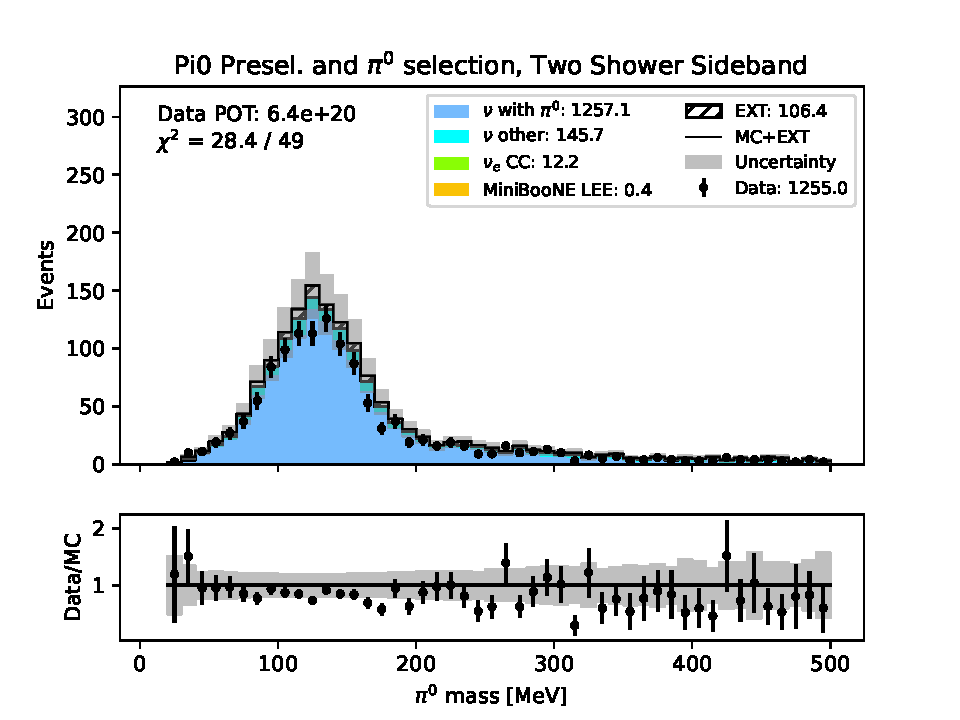
\includegraphics[width=\linewidth]{technote/Sidebands/Figures/TwoShowerSideband/two_shr_sideband_pi0_mass_Y_corr_run123_PI0_PI0.pdf}
        \caption{Reconstructed $\pi^0$ mass, runs 1-3.}
    \end{subfigure}%
    \begin{subfigure}{0.33\linewidth}
        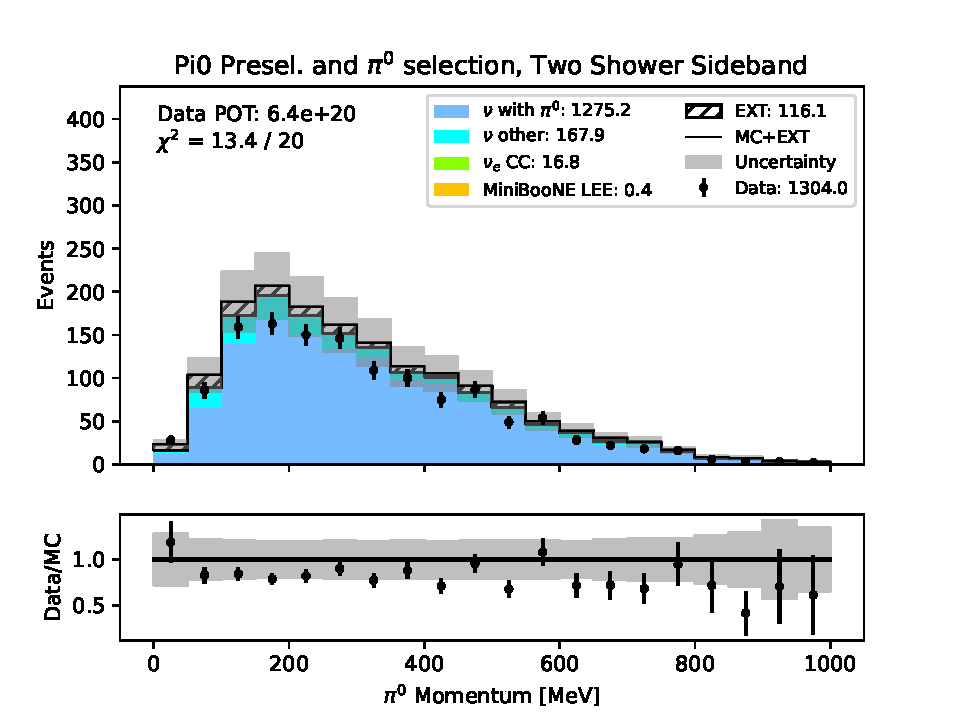
\includegraphics[width=\linewidth]{technote/Sidebands/Figures/TwoShowerSideband/two_shr_sideband_pi0momentum_run123_PI0_PI0.pdf}
        \caption{Reconstructed $\pi^0$ momentum, runs 1-3.}
    \end{subfigure}%
    \begin{subfigure}{0.33\linewidth}
        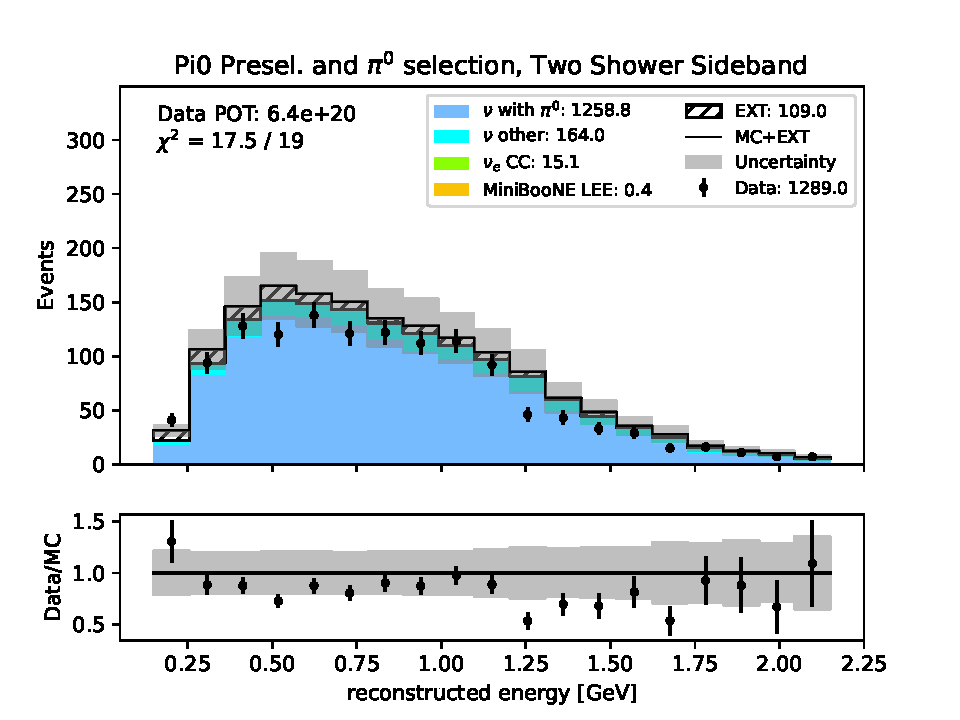
\includegraphics[width=\linewidth]{technote/Sidebands/Figures/TwoShowerSideband/two_shr_sideband_reco_e_run123_PI0_PI0.pdf}
        \caption{Reconstructed neutrino energy, runs 1-3.}
    \end{subfigure}
    \begin{subfigure}{0.33\linewidth}
        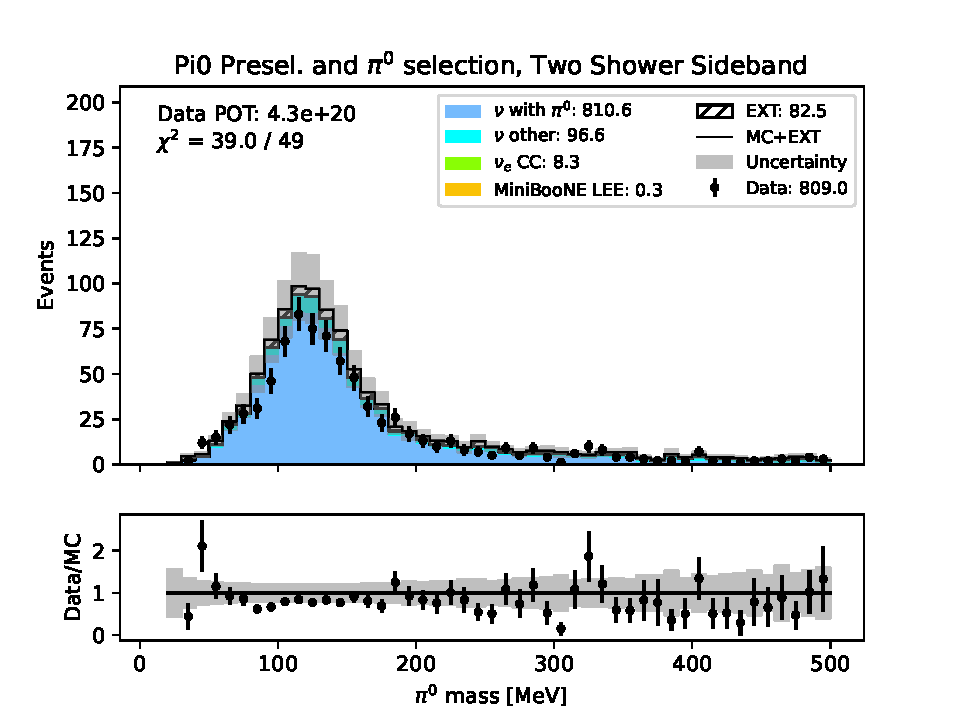
\includegraphics[width=\linewidth]{technote/Sidebands/Figures/TwoShowerSideband/two_shr_sideband_pi0_mass_Y_corr_run4b4c4d5_PI0_PI0.pdf}
        \caption{Reconstructed $\pi^0$ mass, runs 4-5.}
    \end{subfigure}%
    \begin{subfigure}{0.33\linewidth}
        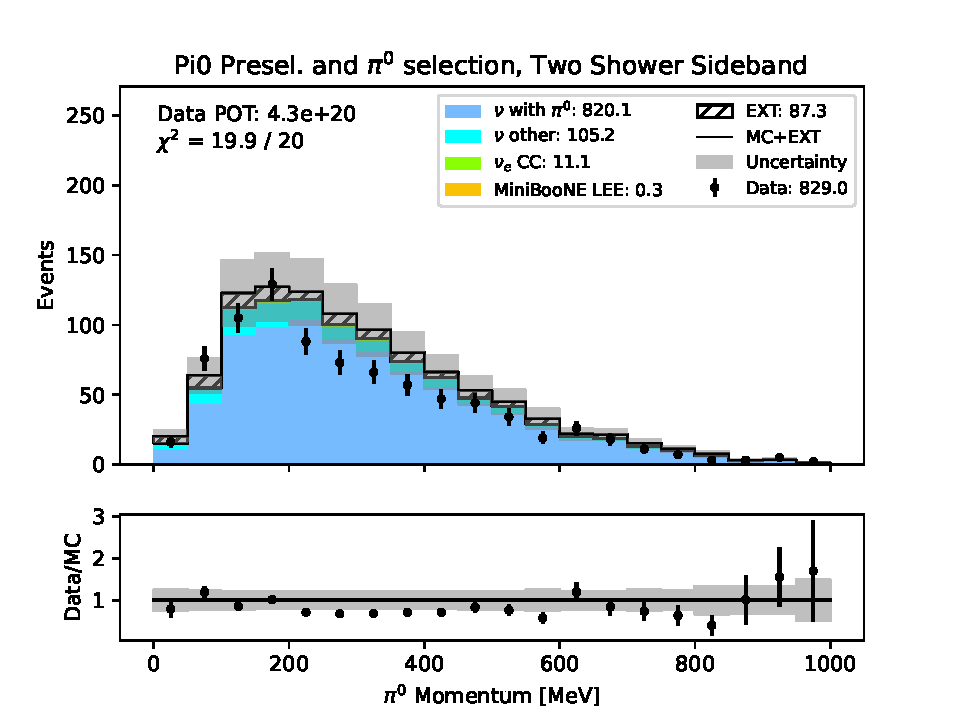
\includegraphics[width=\linewidth]{technote/Sidebands/Figures/TwoShowerSideband/two_shr_sideband_pi0momentum_run4b4c4d5_PI0_PI0.pdf}
        \caption{Reconstructed $\pi^0$ momentum, runs 4-5.}
    \end{subfigure}%
    \begin{subfigure}{0.33\linewidth}
        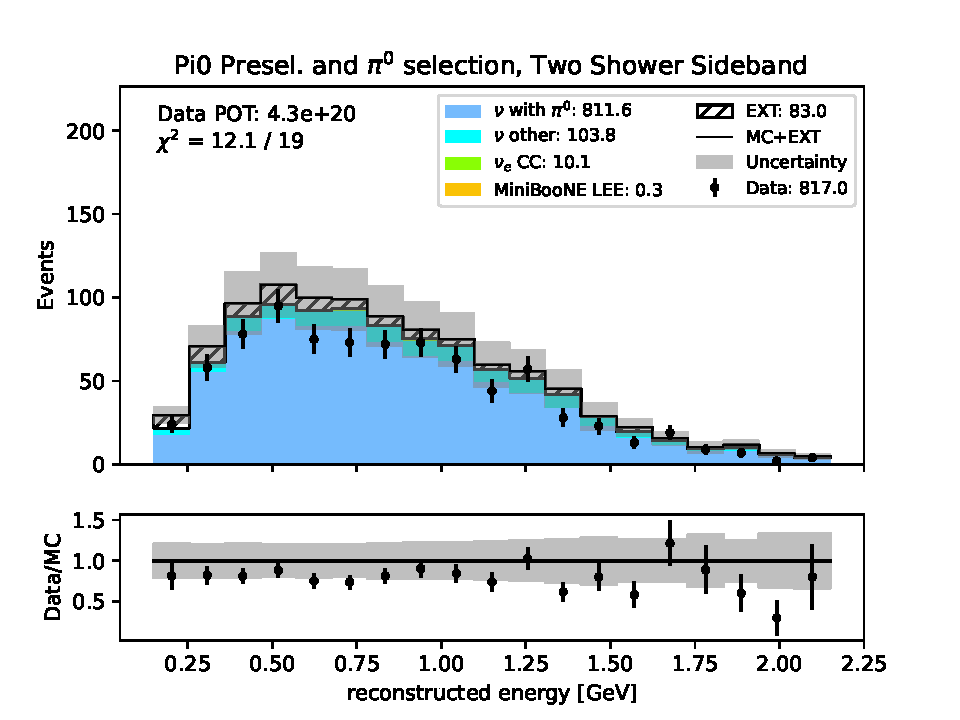
\includegraphics[width=\linewidth]{technote/Sidebands/Figures/TwoShowerSideband/two_shr_sideband_reco_e_run4b4c4d5_PI0_PI0.pdf}
        \caption{Reconstructed neutrino energy, runs 4-5.}
    \end{subfigure}
    \begin{subfigure}{0.33\linewidth}
        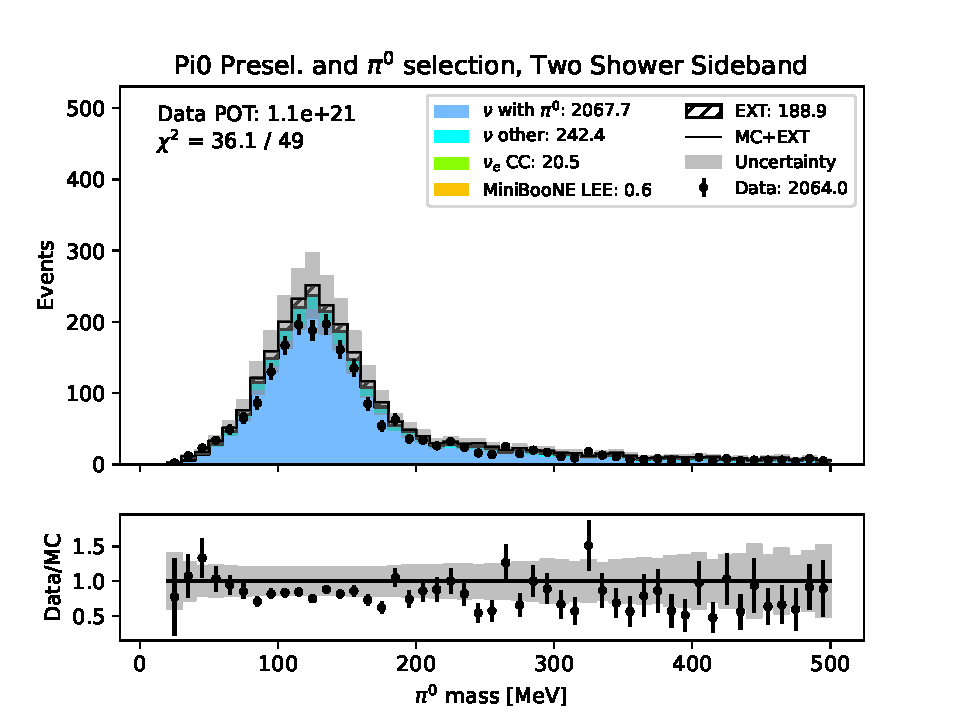
\includegraphics[width=\linewidth]{technote/Sidebands/Figures/TwoShowerSideband/two_shr_sideband_pi0_mass_Y_corr_run1234b4c4d5_PI0_PI0.pdf}
        \caption{Reconstructed $\pi^0$ mass, runs 1-5.}
    \end{subfigure}%
    \begin{subfigure}{0.33\linewidth}
        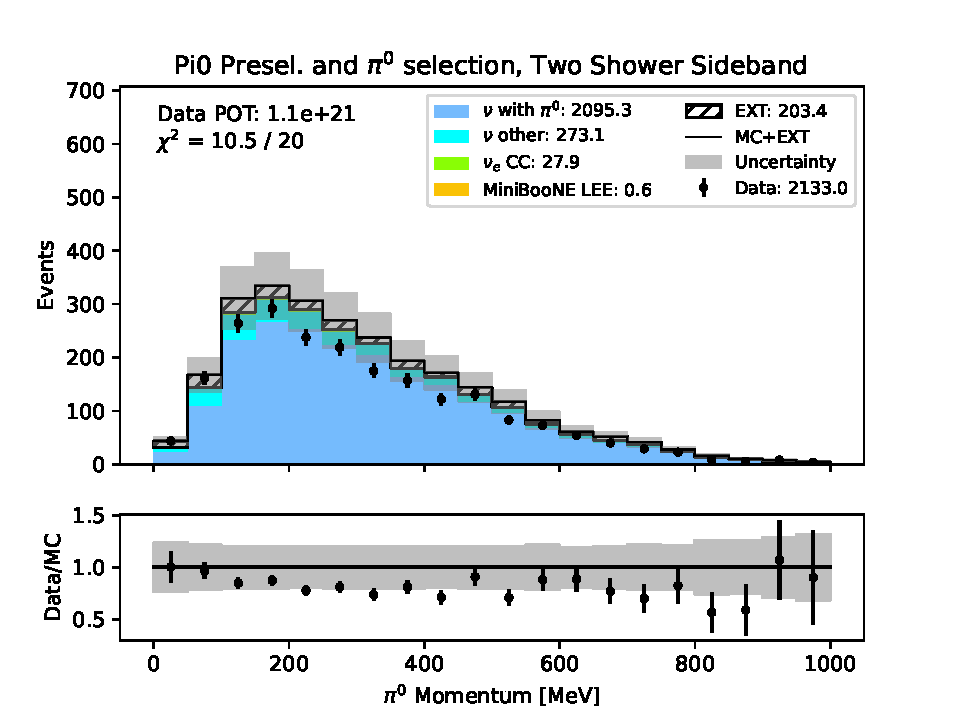
\includegraphics[width=\linewidth]{technote/Sidebands/Figures/TwoShowerSideband/two_shr_sideband_pi0momentum_run1234b4c4d5_PI0_PI0.pdf}
        \caption{Reconstructed $\pi^0$ momentum, runs 1-5.}
    \end{subfigure}%
    \begin{subfigure}{0.33\linewidth}
        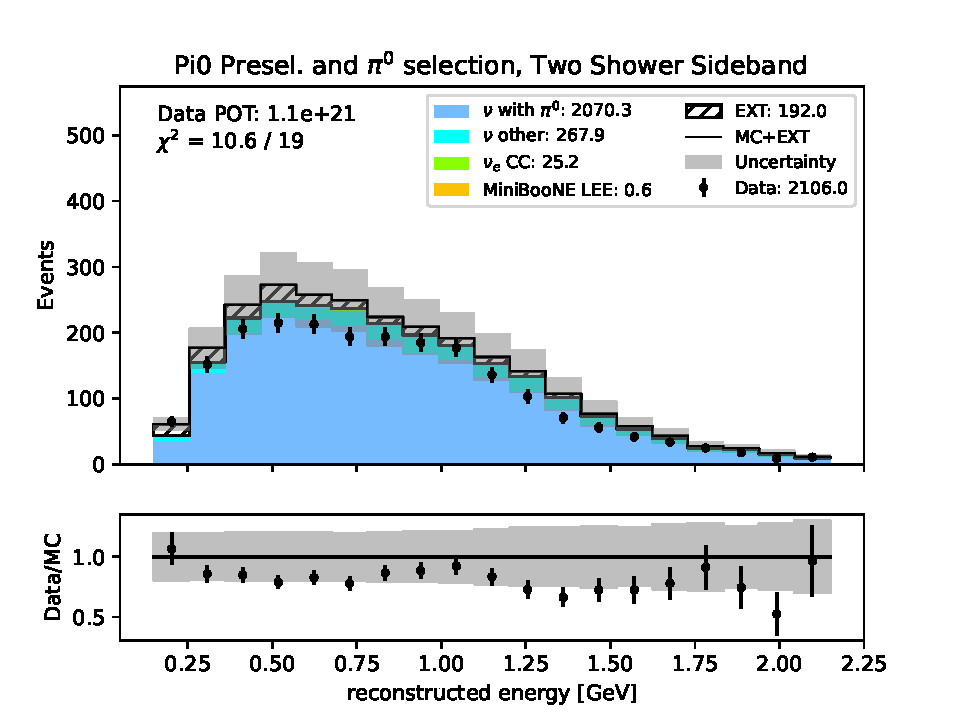
\includegraphics[width=\linewidth]{technote/Sidebands/Figures/TwoShowerSideband/two_shr_sideband_reco_e_run1234b4c4d5_PI0_PI0.pdf}
        \caption{Reconstructed neutrino energy, runs 1-5.}
    \end{subfigure}
    \caption{Data and MC simulation comparisons after applying the full $\pi^0$ selection from Appendix~\ref{appendix:Pi0Selection} to data from the two shower sideband.}
    \label{fig:Pi0Sideband}
\end{figure}